\actTitle{4.7 - Inverse Trigonometric Functions}

\videoLink{Section 4.7 day 1}{https://www.youtube.com/playlist?list=PLYHZK3b8UFw084fqUEZ7lpLyl4MJiCOwu}
%\videoLink{Section 4.7 day 2}{https://www.youtube.com/playlist?list=PLYHZK3b8UFw0JZy4oRGwxyv_LaTgWK5r2}


\noindent \textbf{Topics:}  inverse trig functions\\

\noindent \textbf{Student Learning Outcomes:}
\begin{enumerate}
\item Students will be able to evaluate the inverse trigonometric functions for sine, cosine, and tangent.
\item Students will be able to solve trigonometric equations using inverse trigonometric functions.
\item Students will be able to find the composition of trigonometric and inverse trigonometric functions.
\end{enumerate}

\hrule 

\bigskip

\noindent \underline{Recall:  } A one-to-one function has an inverse function.
\subsection{Evaluate the Inverse Sine Function}

Let's draw a graph of sine and find it's inverse function:
\vfill

   \noindent\colorbox{blue!10}{%
   \parbox{\dimexpr\linewidth}%
   {%
     \textbf{The inverse sine function.}

     The \textbf{arcsine} function, denoted $\sin^{-1}(x)$, is the
     inverse of the sine function on a limited domain, $y=\sin(x)$,
     $-\frac{\pi}{2} \leq x \leq \frac{\pi}{2}$. On the limited
     domain, $-\frac{\pi}{2} \leq x \leq \frac{\pi}{2}$ the following
     relationships are equivalent:
     \begin{eqnarray*}
       \begin{array}{rcl@{\hspace{4em}}rcl}
         y & = & \sin^{-1}(x), & x & = & \sin(y),
       \end{array}
     \end{eqnarray*}
     and $-1 \leq y \leq 1$. 

     }
 }

\noindent Domain:\\[.5in]
\noindent Range:\\

\newpage
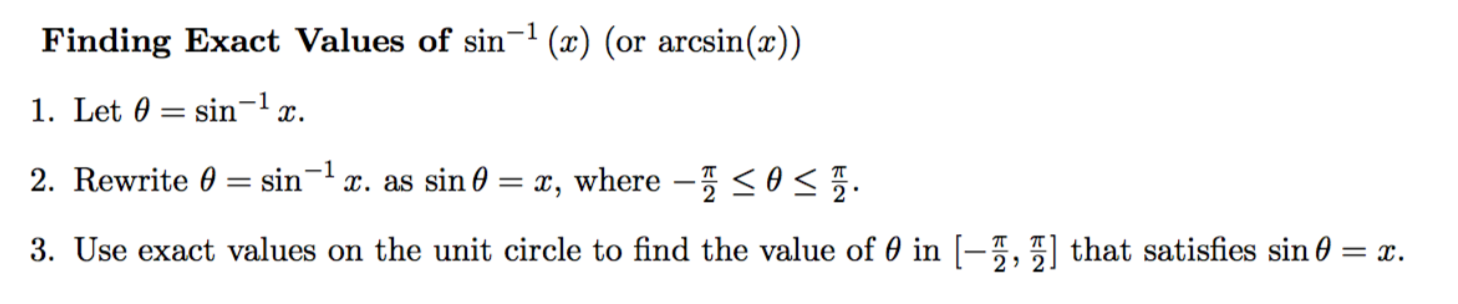
\includegraphics[scale=.7]{findingsineinverse}\\




\begin{enumerate}
\vspace{-.1in}
\item Find the exact values of an inverse function:

\begin{enumerate} 
\item $\displaystyle \sin^{-1}\left(\frac{1}{2}\right)=$\\[.5in]

\item $\displaystyle \sin^{-1}\left(\frac{\sqrt{3}}{2}\right)=$\\[.5in]

\item $\displaystyle \sin^{-1}\left(-\frac{1}{2}\right)=$\\[.5in]
\end{enumerate}




\subsection{Evaluate the Inverse Cosine Function}

Let's draw a graph of cosine and find it's inverse function:
\vfill

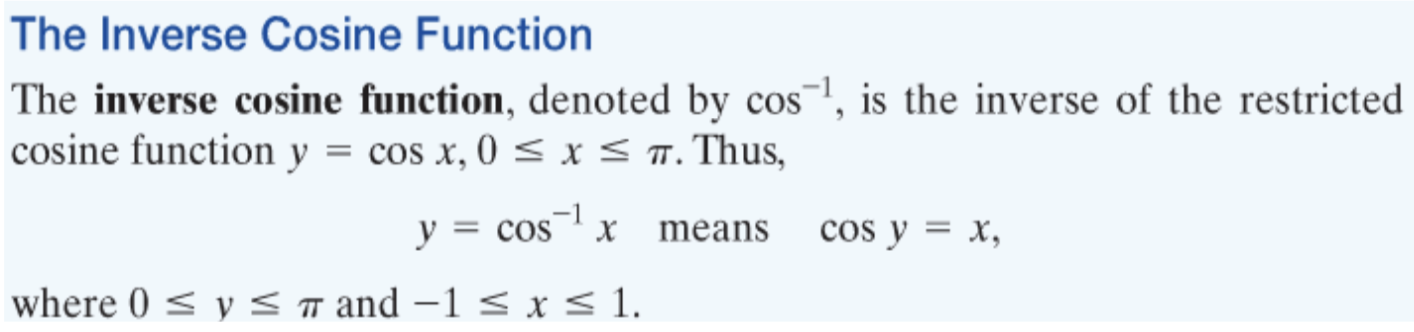
\includegraphics[scale=.7]{cosineinverse}\\
\noindent Domain:\\[.5in]
\noindent Range:\\

\newpage
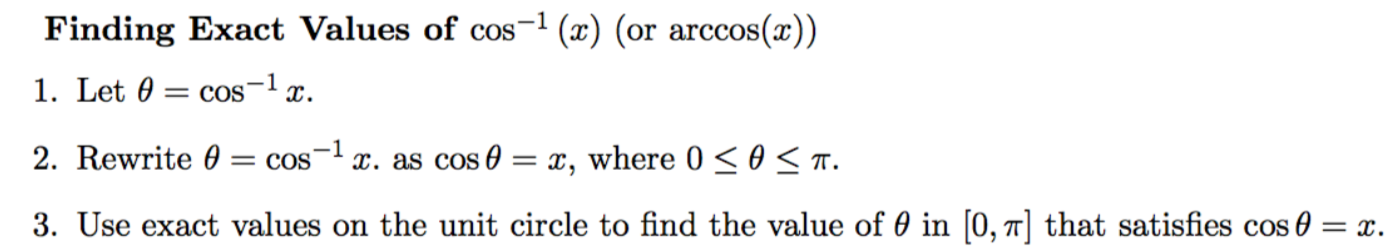
\includegraphics[scale=.7]{findingcosineinverse}\\




\vspace{-.1in}
\item Find the exact values of an inverse function:
 \begin{enumerate}
\item $\displaystyle \cos^{-1}\left(\frac{\sqrt{3}}{2}\right)=$\\[.5in]

\item $\displaystyle \cos^{-1}\left(-\frac{\sqrt{2}}{2}\right)=$\\[.5in]

\item $\displaystyle \cos^{-1}\left(\frac{1}{2}\right)=$\\[.5in]

\end{enumerate}




\subsection{Evaluate the Inverse Tangent Function}

Let's draw a graph of tangent and find it's inverse function:
\vfill

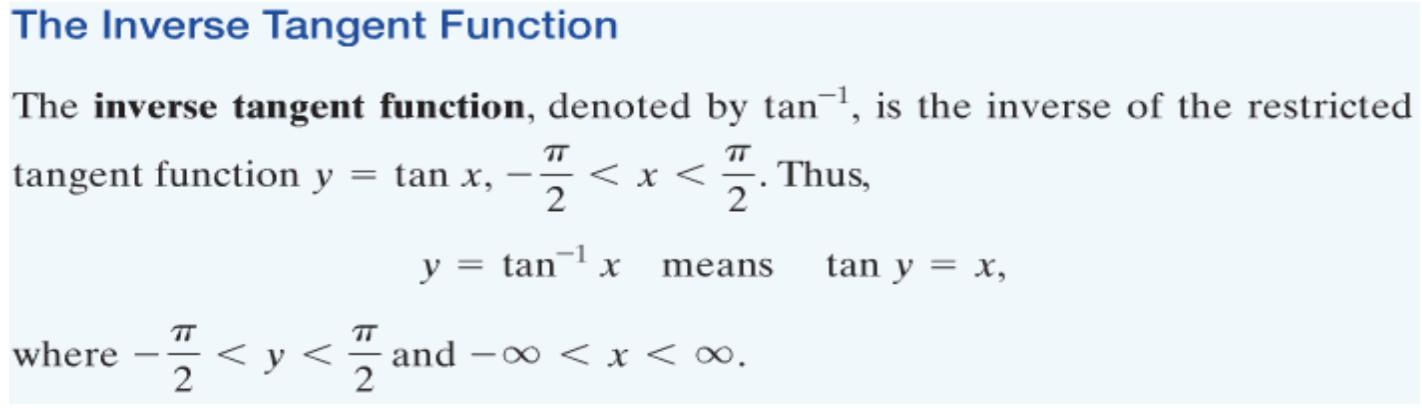
\includegraphics[scale=.7]{tangentinverse}\\
\noindent Domain:\\[.5in]
\noindent Range:\\

\newpage
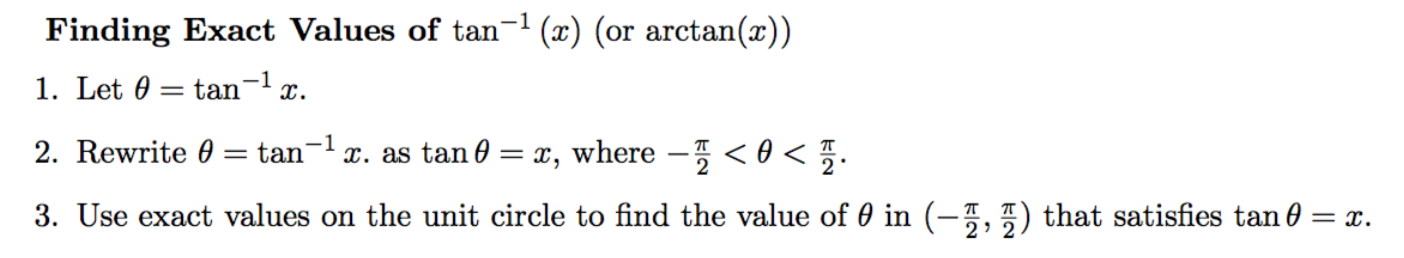
\includegraphics[scale=.7]{findingtangentinverse}\\




\vspace{-.1in}
\item Find the exact values of an inverse function:
 \begin{enumerate}
\item $\displaystyle \tan^{-1}\left(\frac{\sqrt{3}}{3}\right)=$\\[.5in]

\item $\displaystyle \tan^{-1}(0)=$\\[.5in]

\item $\displaystyle \tan^{-1}(1)=$\\[.5in]

\end{enumerate}


\subsection{Approximate Inverse Trigonometric Functions on a Calculator} ~

\item Use a calculator to find the value of each expression rounded to 2 decimal places in radians and degrees.
\begin{enumerate}
\item $\sin^{-1}(.7)=$\\
\item $\cos^{-1}(-.47)=$\\
\item $\tan^{-1}(-14)=$\\
\end{enumerate}


\newpage

\subsection{Inverse Properties of Trigonometric Functions} ~

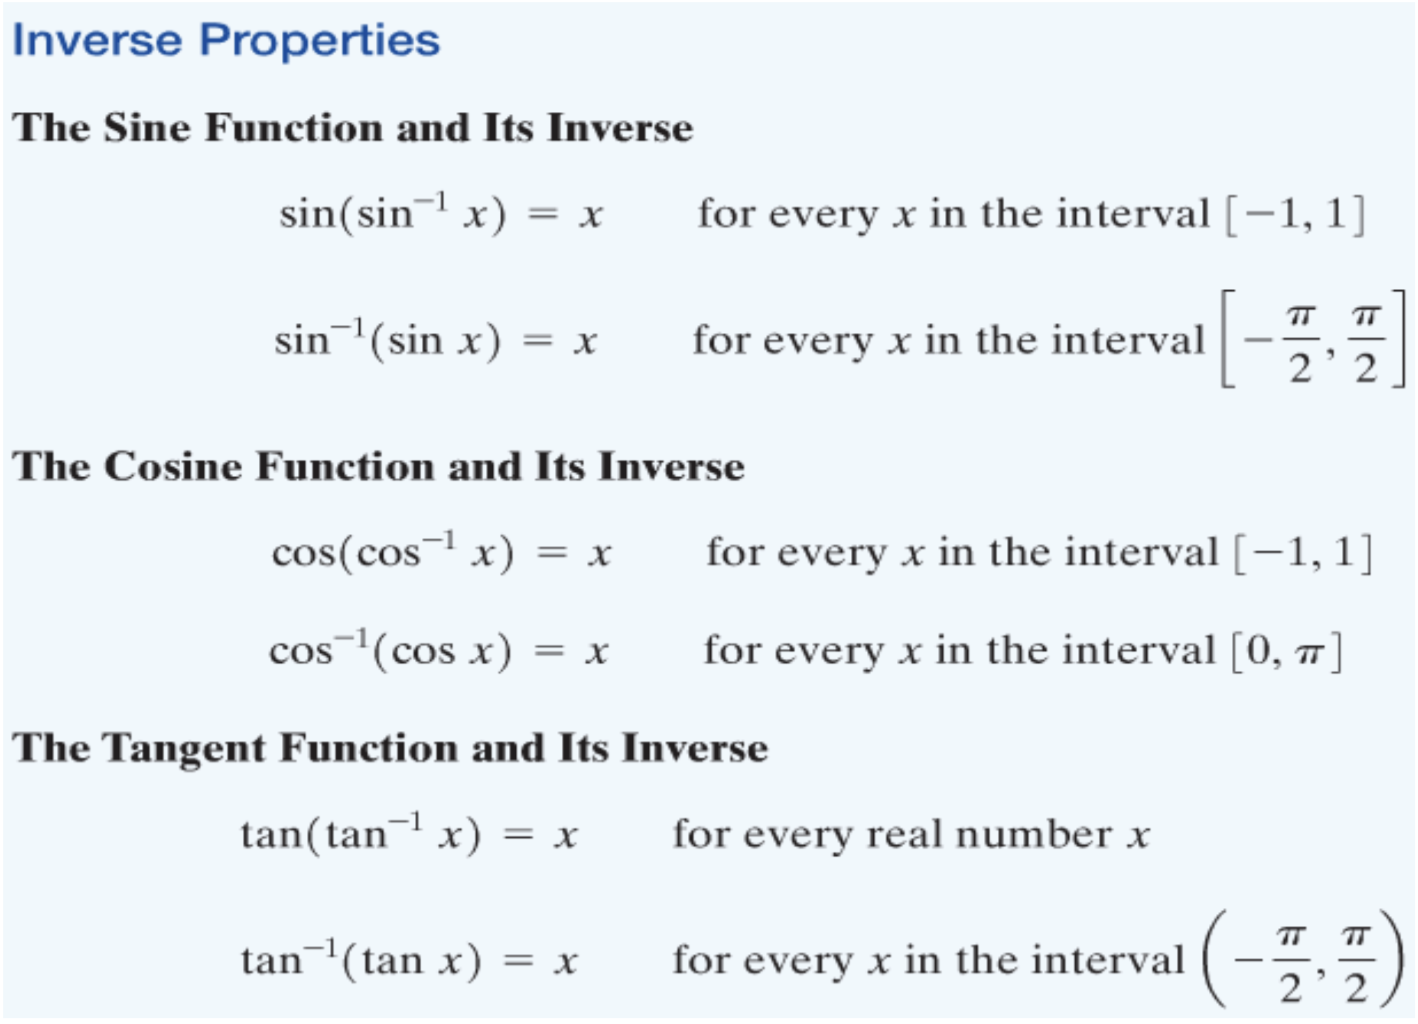
\includegraphics[scale=.7]{inverseprops}

\item Find the exact value of the expression.  Do not use a calculator.
\begin{enumerate}
\item $\displaystyle \cos\left(\cos^{-1}(-0.4)\right)$\vfill
\item  $\displaystyle \sin^{-1}\left(\cos\left(\frac{\pi}{12}\right)\right)$\vfill
\item $\displaystyle \sin^{-1}\left(\sin\left(\frac{3\pi}{12}\right)\right)$\vfill
\newpage
\item $\displaystyle \tan\left(\tan^{-1}(11)\right)$\vfill
\item  $\displaystyle \tan^{-1}\left(\tan\left(-\frac{\pi}{4}\right)\right)$\vfill
\item  $\displaystyle \sin^{-1}\left(\sin(\pi)\right)$\vfill
\item $\displaystyle \sin\left(\sin^{-1}\left(\pi\right)\right)$\vfill
\end{enumerate}

\subsection{Composing Trigonometric and Inverse Trigonometric  Functions} ~

\item Use a sketch to find the exact value of each expression.
\begin{enumerate}
\item $\displaystyle \cos\left(\sin^{-1}\left(\frac{24}{26}\right)\right)$\vfill
\vfill
\newpage
\item $\displaystyle \tan\left(\cos^{-1}\left(-\frac{10}{26}\right)\right)$\vfill
\item $\displaystyle \sec\left(\sin^{-1}\left(-\frac{1}{6}\right)\right)$\vfill
\end{enumerate}


\end{enumerate}
\vfill
\noindent \textbf{Student Learning Outcomes Check}

\begin{enumerate}
\item Can you evaluate the inverse trigonometric functions for sine, cosine, and tangent?
\item Can you solve trigonometric equations using inverse trigonometric functions?
\item Are you able to find the composition of trigonometric and inverse trigonometric functions?

\end{enumerate}

\noindent \textbf{If any of your answers were no, please ask about these topics in class.}

